%%%%%%%%%%%%%%%%%%%%%%%%%%%%%%%%%%%%%%%%%%%%%%%%%%%%%%%%%%%%%%%%%%%%%%%%%%%%%%%
\documentclass[12pt,a4paper,notitlepage,final]{article}
% cestina a fonty
\usepackage[czech]{babel}
\usepackage[T1]{fontenc}
\usepackage[utf8]{inputenc}
% obrazky
\usepackage[dvipdf]{graphicx}
% velikost stranky
\usepackage[top=3.5cm, left=2.5cm, text={17cm, 24cm}, ignorefoot]{geometry}
%% cislovani objektu
\usepackage{chngcntr}
\counterwithin{figure}{section}
% balicky pro odkazy
\usepackage{color}
\usepackage{url}
\usepackage[unicode,colorlinks,hyperindex,plainpages=false,pdftex,linktoc=all]{hyperref}
\definecolor{urlBlue}{rgb}{0.1,0,0.7}
\definecolor{citeGreen}{rgb}{0,0.5,0}
\definecolor{linkRed}{rgb}{0.8,0.1,0.1}
\definecolor{fileSteelBlue}{rgb}{0,0.2,0.4}
\hypersetup{
    linkcolor=linkRed,          % color of internal links
    citecolor=citeGreen,        % color of links to bibliography
    filecolor=fileSteelBlue,    % color of file links
    urlcolor=urlBlue            % color of external links
}
\usepackage{color,colortbl}
\usepackage{multirow}

\usepackage{amsfonts}
\usepackage{amsmath}

\usepackage{pgfplots}
\usepackage{pgfplotstable}
\pgfplotsset{compat=1.10}

\definecolor{tableGray}{rgb}{0.8,0.8,0.8}
% mezera mezi odstavci
\setlength{\parskip}{0.5\baselineskip}%

\usepackage{listingsutf8}
\usepackage{lineno}

% \renewcommand\lstlistingname{Pseudokód}
% \renewcommand\lstlistlistingname{Pseudokód}
% \def\lstlistingname{Pseudokód}
% \lstset{ %
% language=C,                   % the language of the code
% basicstyle=\footnotesize,       % the size of the fonts that are used for the code
% numbers=left,                   % where to put the line-numbers
% numberstyle=\footnotesize,      % the size of the fonts that are used for the line-numbers
% stepnumber=1,                   % the step between two line-numbers. If it's 1, each line
%                                 % will be numbered
% numbersep=-10pt,                % how far the line-numbers are from the code
% backgroundcolor=\color{white},  % choose the background color. You must add \usepackage{color}
% showspaces=false,               % show spaces adding particular underscores
% showstringspaces=false,         % underline spaces within strings
% showtabs=false,                 % show tabs within strings adding particular underscores
% frame=tb,                       % adds a frame around the code
% tabsize=2,                      % sets default tabsize to 2 spaces
% captionpos=b,                   % sets the caption-position to bottom
% breaklines=true,                % sets automatic line breaking
% breakatwhitespace=false,        % sets if automatic breaks should only happen at whitespace
% title=\lstname,                 % show the filename of files included with \lstinputlisting;
%                                 % also try caption instead of title
% escapeinside={\%*}{*)},         % if you want to add a comment within your code
% morekeywords={CODE,..., fakulta},            % if you want to add more keywords to the set
% commentstyle=\color{gray}\upshape
% }

\lstset{
  inputencoding=utf8,
  frame=single,
  title=\lstname
}

\begin{document}

\begin{center}
  \begin{Large}
    Kódování a komprese dat \\
  \end{Large}
  \begin{large}
    Převod grafického formátu GIF do formátu BMP
  \end{large}
\end{center}

\begin{center}
  Ondřej Janošík <xjanos12@stud.fit.vutbr.cz>
\end{center}

\section{Knihovna \texttt{gif2bmp}}

Knihovna poskytuje funkci pro převod obrázků z~formátu \textit{GIF} do
formátu \textit{BMP}.
Nejsou podporovány animované ani průhledné obrázky. V~případě, že \textit{GIF}
obsahuje více snímků, je extrahován pouze první. Obrázky s~prokládanými řádky
podporovány jsou.

Rozhraní knihovny je definováno v~souboru \texttt{gif2bmp.h} a knihovnu lze
linkovat s~jazykem C\footnote{Linkování s~jazykem C vyžaduje přilinkování
standardní knihovny jazyka C++ (\texttt{-lstdc++}).} i~C++. Knihovna definuje
funkci \texttt{gif2bmp()} (kód \ref{lst:gif2bmp}) která provádí samotný převod.
Ta bere jako parametry ukazatel na strukturu \texttt{tGIF2BMP}
(kód \ref{lst:tgif2bmp}) a~dále ukazatel na popisovače vstupního a výstupního
souboru.

Návratové kódy funkce \texttt{gif2bmp()} jsou popsány v~ukázce
kódu~\ref{lst:return_codes}.
Funce vrací hodnotu \texttt{GIF2BMP\_OK} při úspěšném provedení a~hodnotu
\texttt{GIF2BMP\_ERROR}, pokud dojde k~chybě (např. nevalidní obrázek, či chyba
čtení ze souboru). Po úspěšném provedení obsahuje struktura \texttt{tGIF2BMP}
velikost souboru s~obrázkem \textit{GIF} a \textit{BMP}.

\lstinputlisting[language=C, firstline=34, lastline=34,
  caption={Deklarace funce \texttt{gif2bmp()}.},
  label={lst:gif2bmp}
  ]{lst/gif2bmp.h}

\lstinputlisting[language=C, firstline=24, lastline=27,
  caption={Definice typu \texttt{tGIF2BMP}.},
  label={lst:tgif2bmp},
  ]{lst/gif2bmp.h}

\lstinputlisting[language=C, firstline=29, lastline=32,
  caption={Definice návratových hodnot.},
  label={lst:return_codes},
  ]{lst/gif2bmp.h}

\section{Dekomprese formátu GIF}

Obrázkový formát GIF existuje ve dvou verzích: \textit{GIF87a} a \textit{GIF89a}.
Oproti verzi \textit{GIF87a} má verze \textit{GIF89a} navíc rozšiřující bloky
(extensions). Tyto bloky umožňují přidávat informace specifické pro konkrétní
aplikaci, komentáře, vykreslovat do obrázku text a řídit průhlednost a animaci
obrázku. Pro účely knihovny jsou tyto bloky pouze detekovány a následně
ignorovány.

\subsection{LZW dekomprese}

Formát \textit{GIF} používá kompresní algoritmus \textit{LZW}. Avšak nejedná
se o~běžný algoritmus \textit{LZW}, nýbrž algoritmus upravený pro potřeby
formátu \textit{GIF}. Úprava spočívá v~použití proměnlivé délky kódového slova,
která může nabývat hodnot od 3 do 12.

\begin{figure}
  \centering
  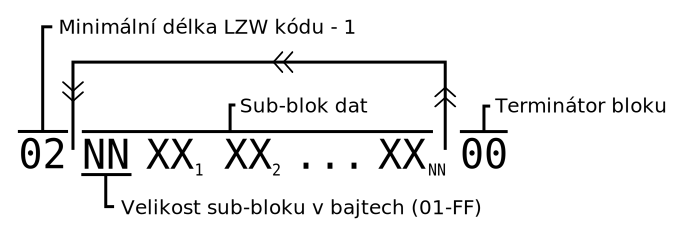
\includegraphics[width=10cm, keepaspectratio]{img/image-data}
  \caption{Struktura bloku obrazových dat.}
  \label{img:image-data}
\end{figure}

Dekomprese začíná ve chvíli, kdy program narazí na blok obrazových dat
(obrázek \ref{img:image-data}). První bajt (\texttt{lzwInitialCodeSize})
určuje minimální délku kódu \\ (\texttt{lzwCodeSize = lzwInitialCodeSize + 1}),
počáteční velikost tabulky kódů (\texttt{1 <{}< lzwCodeSize}) a hodnoty
speciálních kódů \textit{Clear code} (\texttt{CC = 1 <{}< lzwInitialCodeSize}) a
\textit{End of information code} (\texttt{EOI = CC + 1}).

\begin{lstlisting}[language=C,
  caption={Pseudokód pro dekódování LZW dat.},
  label={lst:lzw_decode},
  ]
  Start:
  Inicializace tabulky kodu
    Nacti CODE    // CODE - hodnota kodu
    Zapis {CODE}  // {CODE} - obsah tabulky kodu na indexu CODE
    while(lze cist) {
      Nacti CODE
      if(CODE == CC) {
        goto Start
      }
      else if(CODE == EOI) {
        break
      }

      if(CODE je v tabulce) {
        Zapis {CODE}
        K = prvni hodnota v {CODE}
        Pridej {CODE - 1} + K do tabulky
      }
      else {
        K = prvni hodnota v {CODE - 1}
        Zapis {CODE - 1} + K
        Pridej {CODE - 1} + K do tabulky
      }
    }
\end{lstlisting}

Algoritmus dekomprese obrazových dat je popsán pseudokódem~\ref{lst:lzw_decode}.
Vždy když dojde k~překročení velikosti tabulky, navýší se velikost kódu
(\texttt{lzwCodeSize += 1}) a velikost tabulky se zdvojnásobí.
Pokud algoritmus narazí na \textit{Clear code}, hodnota velikosti kódu
i~tabulky se resetuje a algoritmus se opakuje od začátku.
\textit{End of information code} pak explicitně označuje konec bloku obrazových
dat.

\section{Aplikace}

Aplikace \textit{gif2bmp} je terminálová aplikace.
Přepínače aplikace jsou popsány v~tabulce~\ref{tbl:app}.

\begin{table}
  \centering
  \begin{tabular}{| l | l | l |}
    \hline
    \rowcolor[gray]{0.9}
    \textbf{Přepínač}	& \textbf{Parametry}	& \textbf{Popis} \\
    \hline
    -i & INPUT  & Vstupní soubor obrázku (výchozí: stdin). \\
    -o & OUTPUT & Výstupní soubor obrázku (výchozí: stdout). \\
    -l & LOG    & Soubor pro výpis logu. \\
    -h &        & Vypíše nápovědu aplikace.\\ \hline
  \end{tabular}
  \caption{Popis přepínačů aplikace \textit{gif2bmp}.}
  \label{tbl:app}
\end{table}

%%%%%%%%%%%%%%%%%%%%%%%%%%%%%%%%%%%%%%%%%%%%%%%%%%%%%%%%%%%%%%%%%%%%%%%%%%%%%%%

% \newpage
%
% \bibliographystyle{czechiso}
% \begin{flushleft}
% \bibliography{zdroje} % viz. literatura.bib
% \end{flushleft}

\end{document}
